\section{Semantic LSP}%
\label{sec:semantic_lsp}

When developing a LSP, we made sure to follow the state of the art best implementation practices\cite{10.1145/3550355.3552452,10.1145/3563834.3567537,10.1145/3550355.3552452,Bour_2018}.
Semantic LSP is built on top of an entity component system, allowing for even greater seperation of concern than the proposed \textit{Layered Architecture}\cite{10.1145/3550355.3552452}.

Entity component system is a software pattern that involves breaking your program up into Entities, Components, and Systems.
Entities are unique "things", here documents, that are assigned groups of Components, which are then processed using Systems.
Components include the contents of the source file, the location of the source file, the derived triples, etc.
Systems are functions that are grouped in schedules, one system might derive defined owl properties from derived triples and might be present in the \textit{Parse} schedule.
Each language can then add their specific systems into the defined schedules for language specific functionality.
This way common systems are defined once, resulting in a consistent experience over all semantic languages.
Bour et al. state "No spec, no tests"\cite{Bour_2018}, meaning it is difficult to write a useful testsuite for language servers.
User-facing features are not well specified and open for interpretation.
At least common systems act the same way over different semantic languages.

\subsection{Langauge Server schedules}

This section goes into detail on the different systems that are implemented for each schedule of the language server.
Some systems only create components, these components are then used by other systems, potentially in different schedules.
If an expected component is not present, the system will skip that entity, allowing for asynchronously running systems.

\subsubsection*{Parse}

\begin{figure}[!ht]
    \centering
    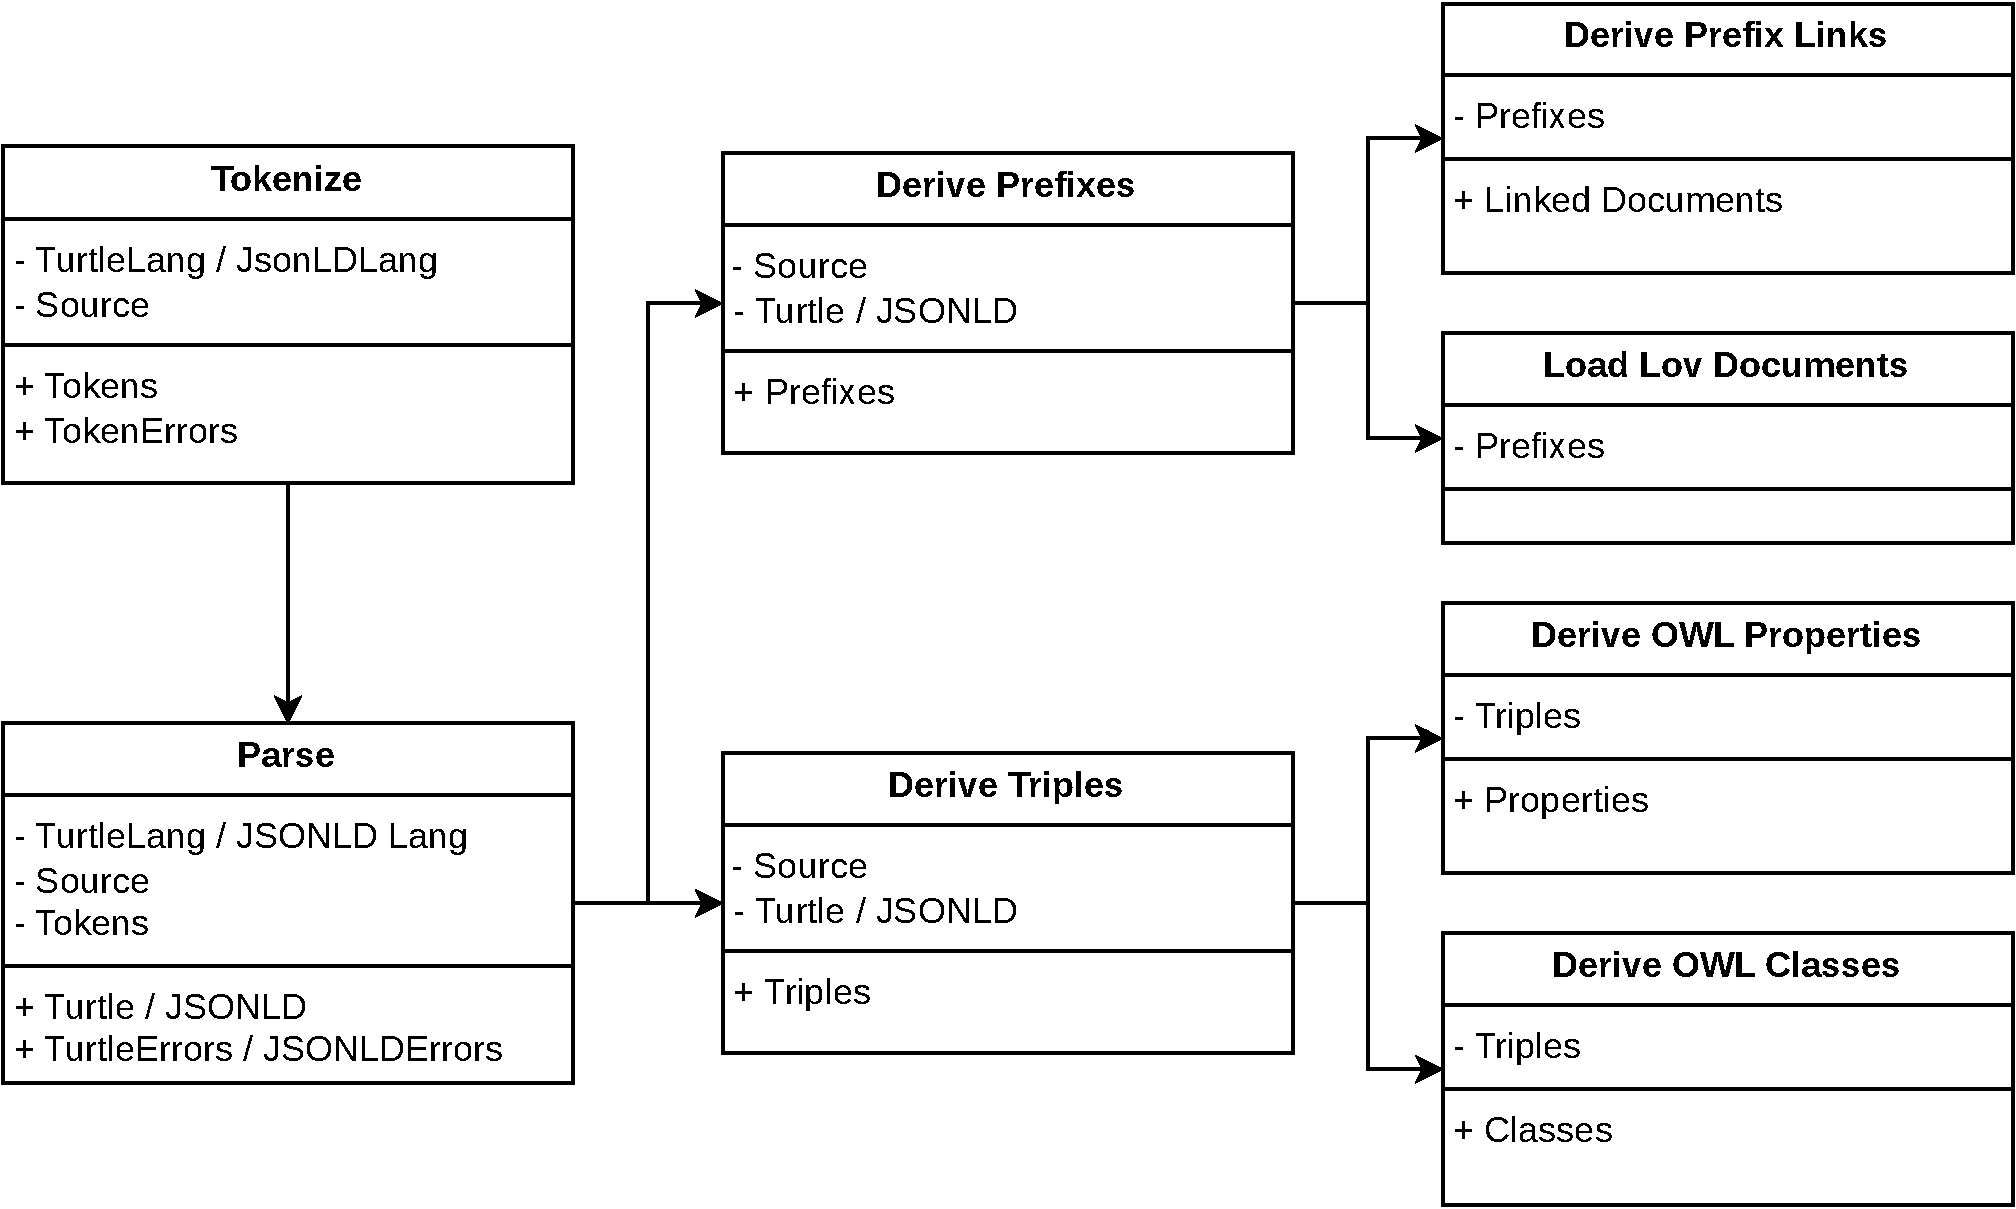
\includegraphics[width=0.95\textwidth]{./images/ParseSchedule.pdf}
    \caption{Visual representation of our example pipeline, 
        loading sensor data from The Things Network into a triple store}\label{fig:Pipeline}
\end{figure}


\subsubsection*{Diagnostics}




\subsubsection*{SemanticHighlighting}

\subsubsection*{Completion}


